\chapter{Conclusion}
\epigraph{Of what a strange nature is knowledge! It clings to a mind when it has once seized on it like a lichen on a rock.}{Mary Shelley, \textit{Frankenstein; or, The Modern Prometheus}}


And thus, we have reached the end. This thesis dealt with the development of a general framework for improving the performance of model-based visual-inertial localization pipelines. We accomplished this by complementing these pipelines with learned probabilistic ‘pseudo-sensors’ that extracted difficult-to-model latent information from sensor data.  We presented four examples of such \textit{pseudo-sensors}. 

\section{Summary of Contributions}

\subsection{Predictive Robust Estimation}

\begin{wrapfigure}{r}{0.3\textwidth}
  \begin{center}
  	\vspace{-25pt}
    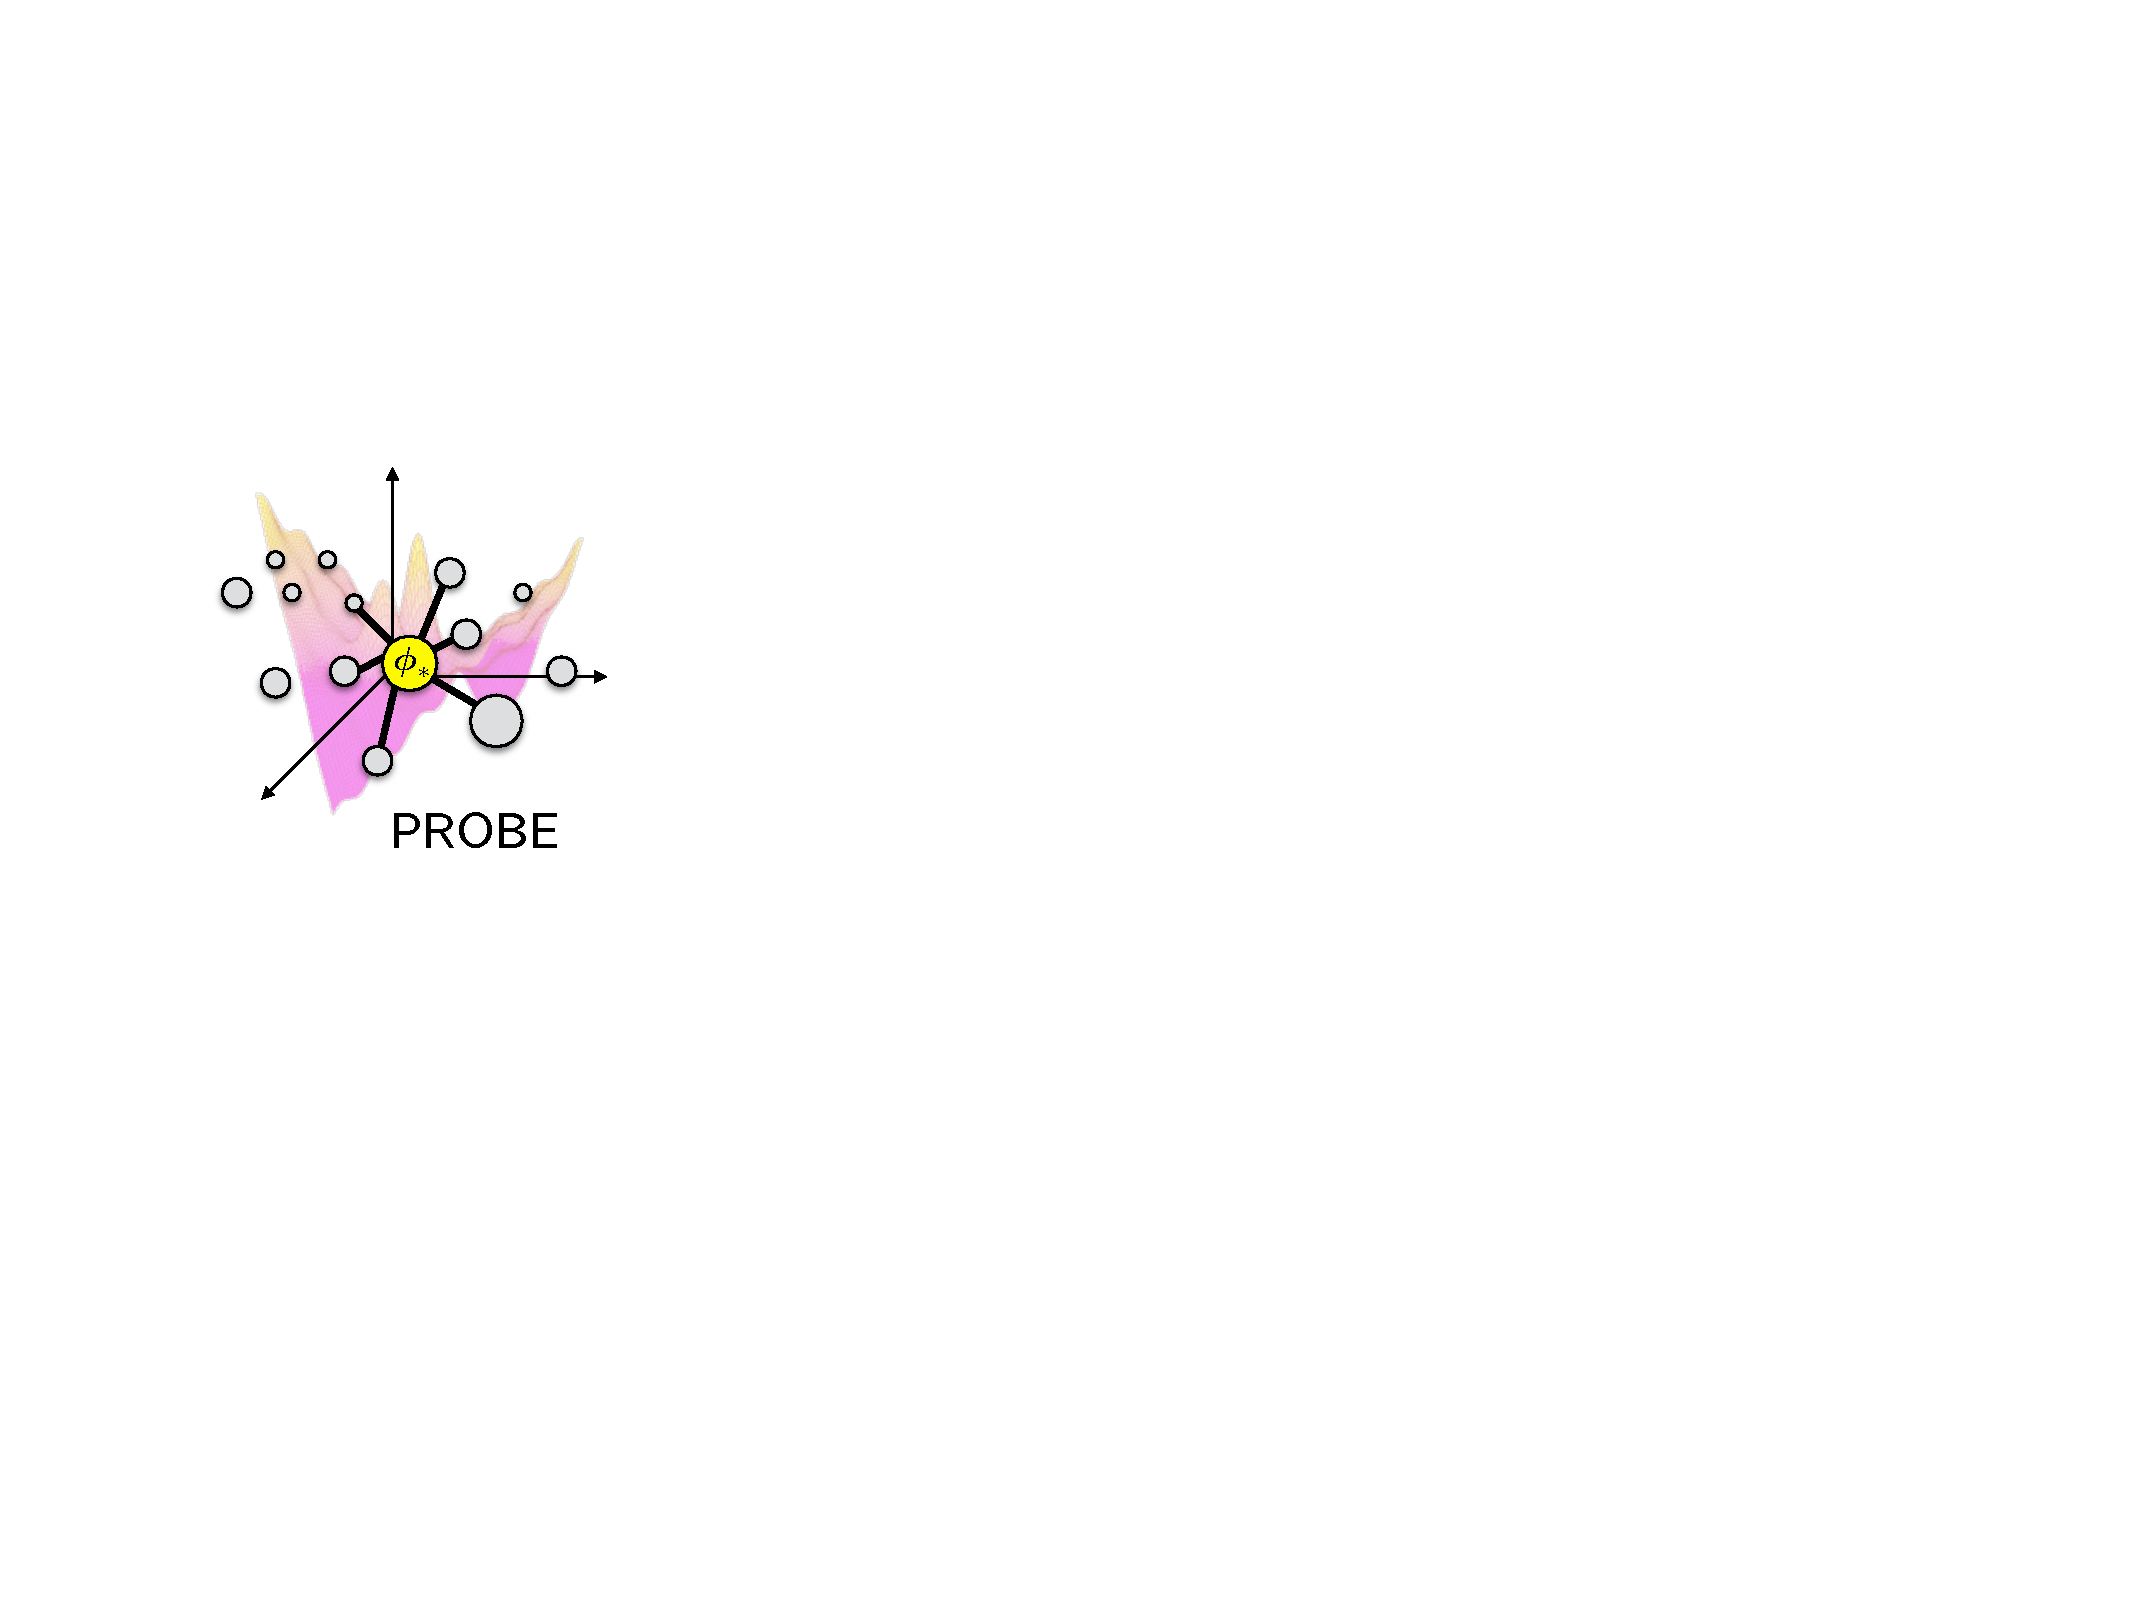
\includegraphics[width=0.28\textwidth]{conclusion/probe}
     \vspace{-25pt}
  \end{center}
  \caption{PROBE (\Cref{ch:probe}).}
  \vspace{-5pt}
\end{wrapfigure}


We began with the pseudo-sensor that used a heteroscedastic noise model to enable predictively robust estimation. PROBE and its follow up PROBE-GK, contributed
\begin{enumerate}
\item a probabilistic model for indirect stereo visual odometry, leading to a predictive robust algorithm for inference on that model,
\item two different approaches to constructing the robust algorithm: one based on k-nearest neighbours, and one based on Generalized Kernel (GK) estimation,
\item a procedure for training our model using pairs of stereo images with known relative transforms, and
\item an iterative, expectation-maximization approach to train our GK model when the relative ground truth egomotion was unavailable.
\end{enumerate}

\noindent A total of three publications associated with PROBE,
\begin{itemize}
	\item \bibentry{2016_Peretroukhin_PROBE-GK}
	\item \bibentry{2015_Peretroukhin_PROBE}
	\item \bibentry{2015_Peretroukhin_Get}.
\end{itemize}


\subsection{Sun BCNN}

\begin{wrapfigure}{r}{0.3\textwidth}
  \begin{center}
  	\vspace{-20pt}
    
\includegraphics[width=0.28\textwidth]{conclusion/sun_bcnn}
     \vspace{-15pt}
  \end{center}
  \caption{Sun BCNN (\Cref{ch:sun-bcnn}).}
  \vspace{-5pt}
\end{wrapfigure}


With Sun-BCNN, we applied learned \textit{pseudo-sensors} to the problem of illumination direction in outdoor environments. In sum, the novel contributions were:
\begin{enumerate}
\item the application of a Bayesian CNN to the problem of sun direction estimation, incorporating the resulting covariance estimates into a visual odometry pipeline; 
\item an empirical demonstration that a Bayesian CNN with dropout layers after each convolutional and fully-connected layer can achieve state-of-the-art accuracy at test time;
\item a loss function that incorporated a 3D unit-length sun direction vector, appropriate for full 6-DOF pose estimation;
\item experimental results on over 30~km of visual navigation data in urban \citep{Geiger2012-fq} and planetary analogue \citep{Furgale2012-kk} environments; 
\item an investigation into the sensitivity of the Bayesian CNN-based sun estimate to cloud cover, camera and environment changes, and measurement parameterization; and
\item open-source software\footnote{\url{https://github.com/utiasSTARS/sun-bcnn-vo}.}.
\end{enumerate}

\noindent Sun-BCNN and its origin in learned sun sensors have three associated publications,
\begin{itemize}
	\item \bibentry{2018_Peretroukhin_Inferring}
	\item \bibentry{2017_Peretroukhin_Reducing}
	\item \bibentry{2017_Clement_Improving}.
\end{itemize}


\subsection{Deep Pose Corrections}

\begin{wrapfigure}{r}{0.3\textwidth}
  \begin{center}
  	\vspace{-20pt}
    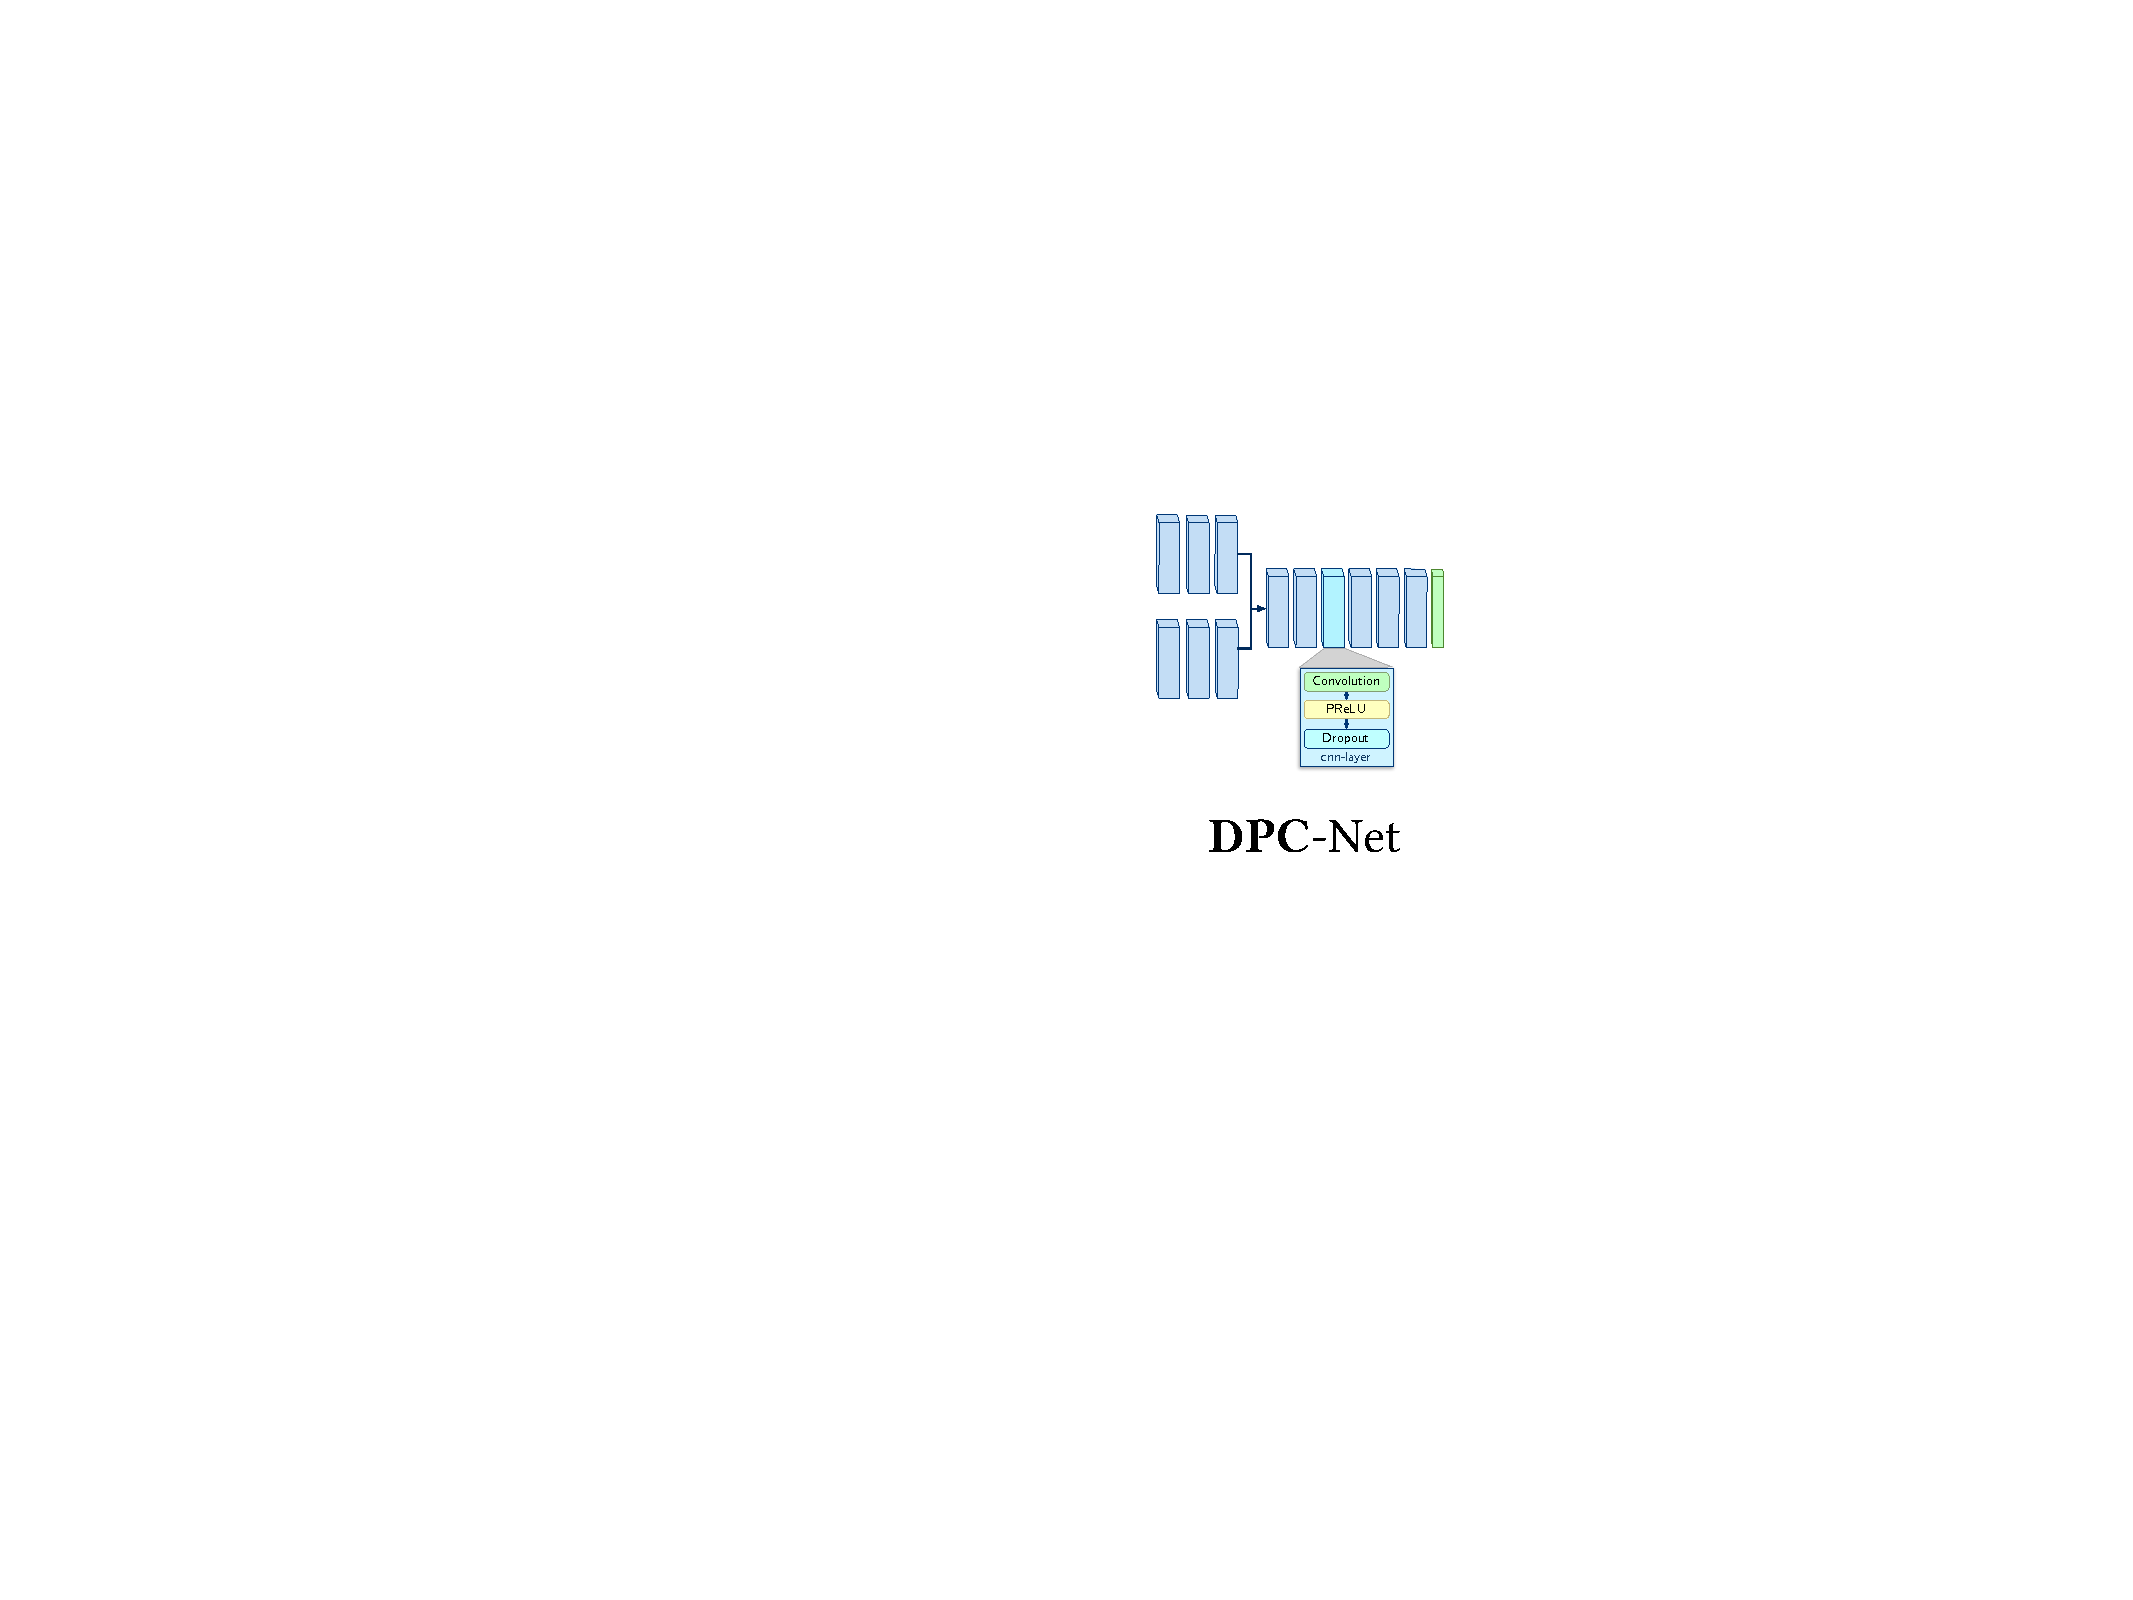
\includegraphics[width=0.28\textwidth]{conclusion/dpc}
     \vspace{-15pt}
  \end{center}
  \caption{DPC-Net (\Cref{ch:dpc}).}
  \vspace{-5pt}
\end{wrapfigure}


Next, we generalized the results of Sun-BCNN to learn full six degree-of-freedom corrections for a particular egomotion pipeline and a given environment with DPC-Net. Our contributions included

\begin{enumerate}
	\item the formulation of a novel deep corrective approach to egomotion estimation,
	\item a novel cost function for deep $\LieGroupSE{3}$ regression that naturally balances translation and rotation errors, and
	\item an open-source implementation of DPC-Net in \texttt{PyTorch}\footnote{See \url{https://github.com/utiasSTARS/dpc-net}.}.
\end{enumerate}

\noindent DPC-Net was published in a journal publication,
\begin{itemize}
	\item \bibentry{2018_Peretroukhin_Deep}.
\end{itemize}


\subsection{Deep Probabilistic Inference of $\LieGroupSO{3}$ with HydraNet}

\begin{wrapfigure}{r}{0.3\textwidth}
  \begin{center}
  	\vspace{-20pt}
    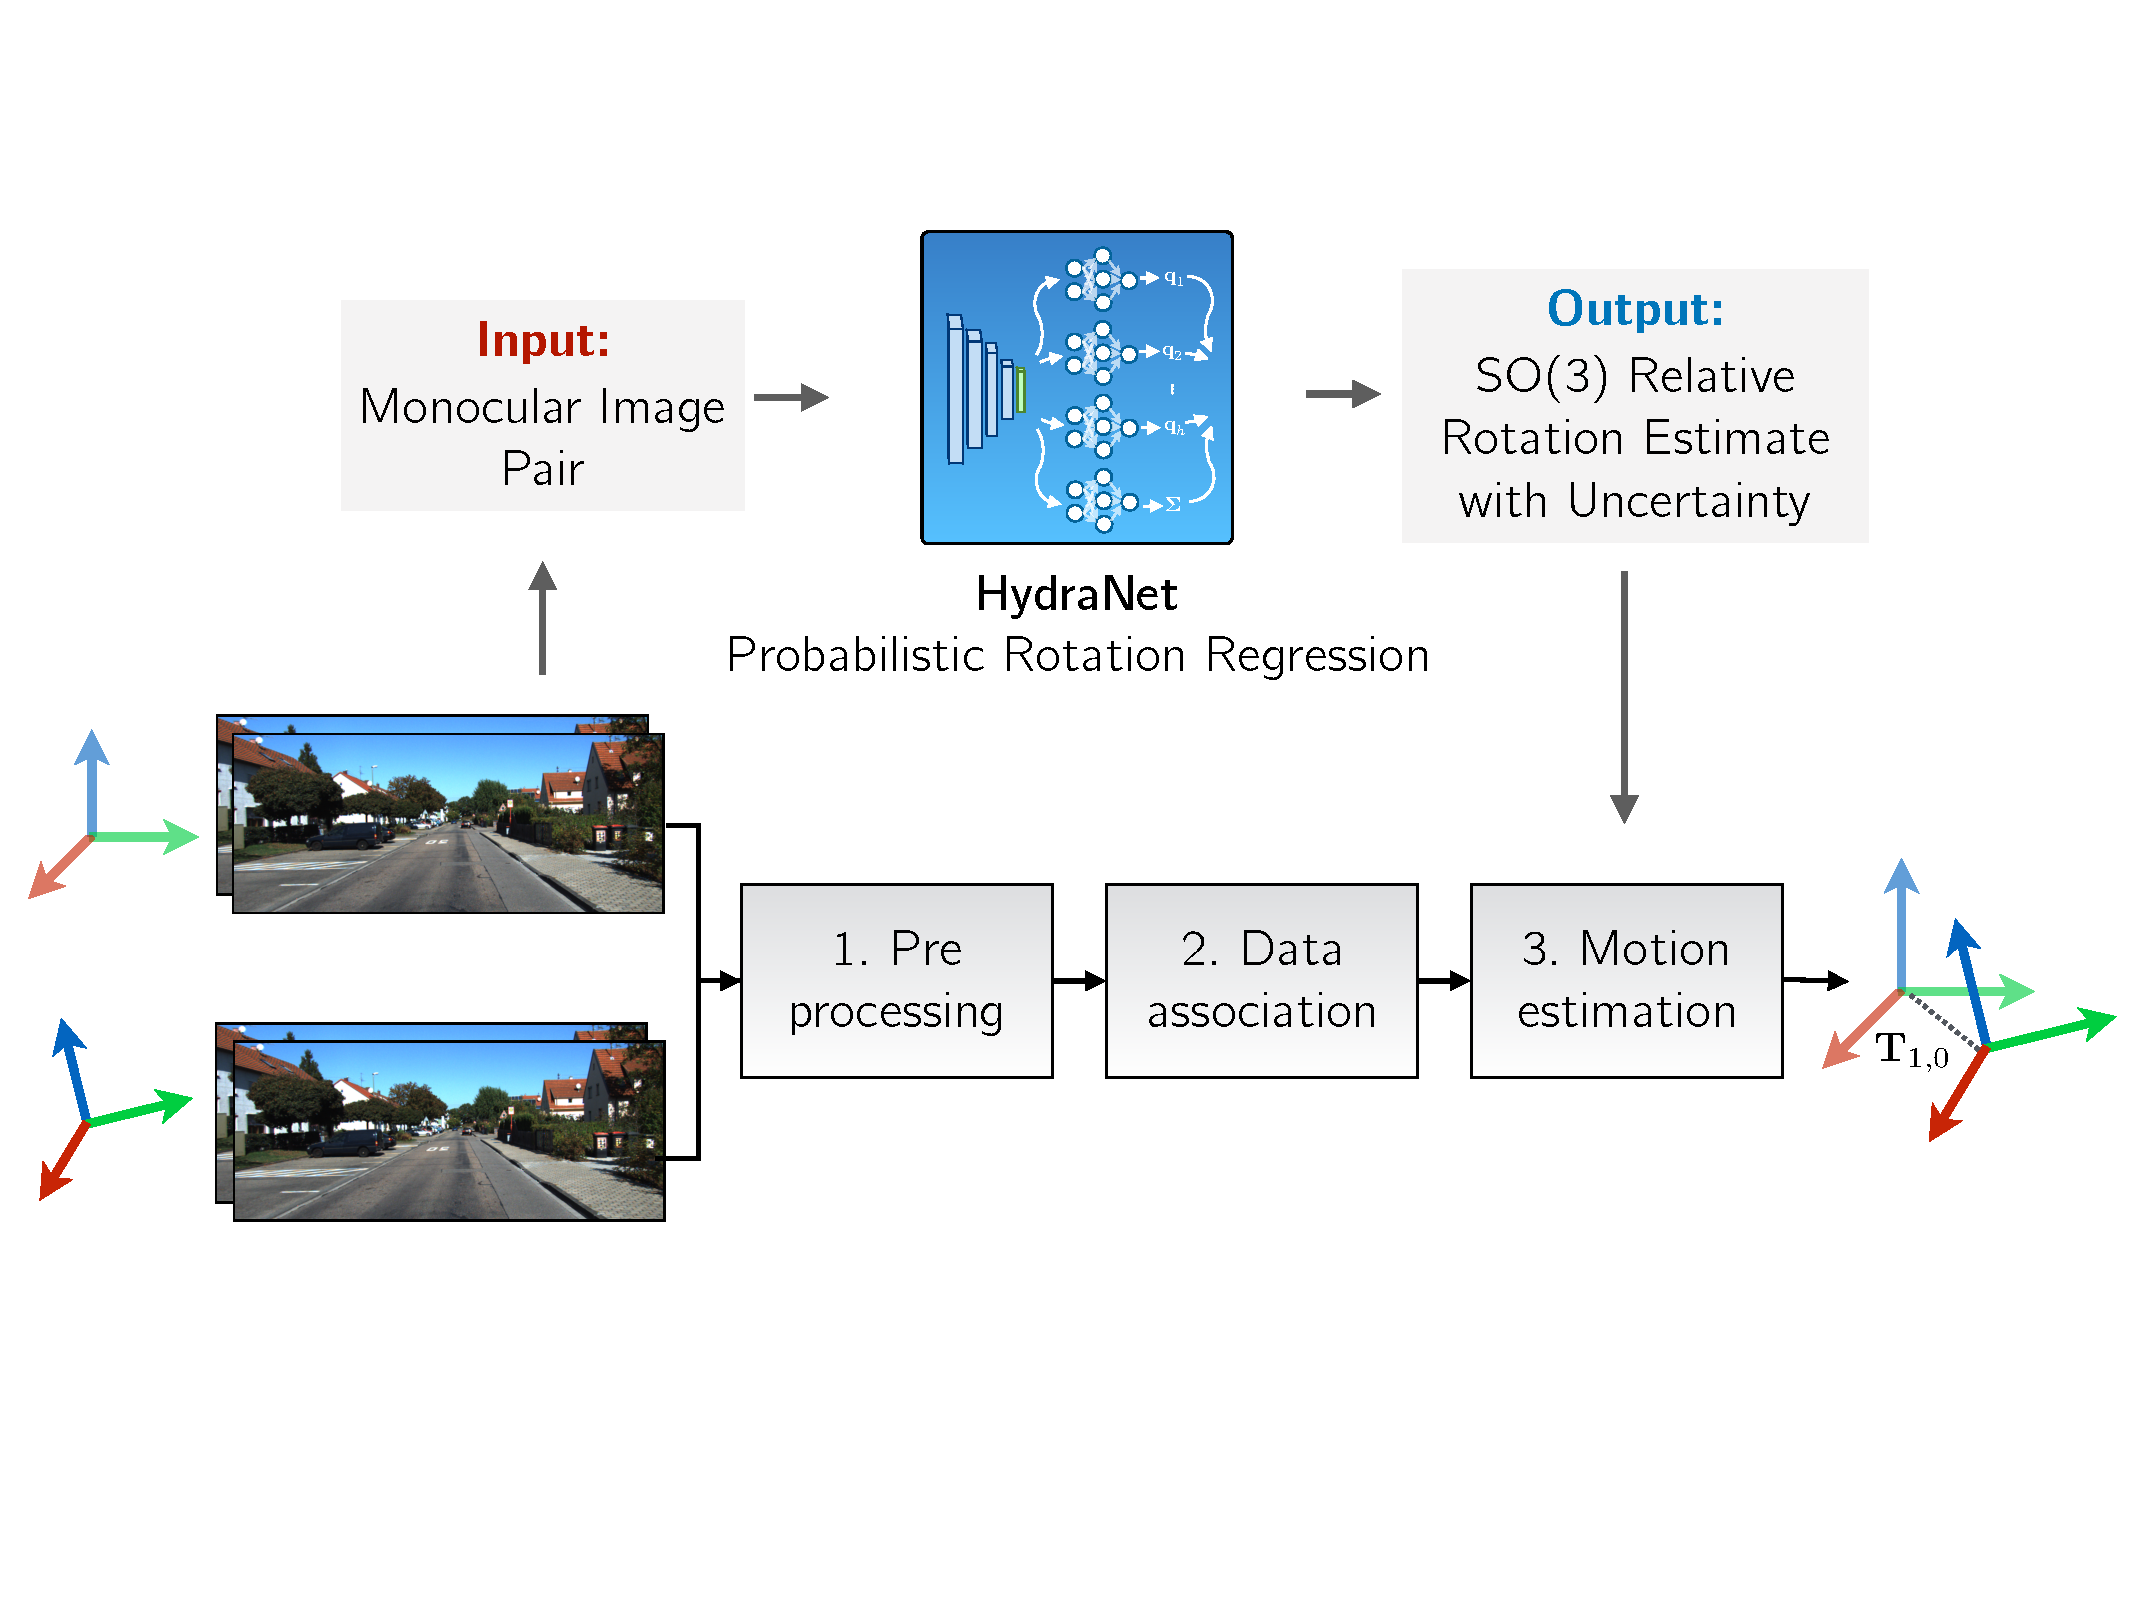
\includegraphics[width=0.28\textwidth]{conclusion/hydranet}
     \vspace{-15pt}
  \end{center}
  \caption{HydraNet (\Cref{ch:hydranet}).}
  \vspace{-5pt}
\end{wrapfigure}


Finally, we applied the lessons of DPC-Net and Sun-BCNN to learning only rotation estimates through a network structure that incorporated both aleatoric and epistemic uncertainty which can be fused with classical pipelines through pose graph optimization. With this work, we contributed
\begin{enumerate}
\item a deep network structure we call \textit{HydraNet} that built on prior work \cite{Lakshminarayanan2017,Osband2016} to produce meaningful uncertainties over unconstrained targets,
\item a loss formulation and mathematical framework that extends HydraNet to means and covariances of the rotation group $\LieGroupSO{3}$,
\item and open source code for $\LieGroupSO{3}$ regression\footnote{\url{https://github.com/utiasSTARS/so3_learning}.}.
\end{enumerate}

\noindent HydraNet was published in a refereed workshop paper,
\begin{itemize}
\item \bibentry{2019_Peretroukhin_Deep}.
\end{itemize}


\section{Future Work}

\begin{figure}
\begin{center}
		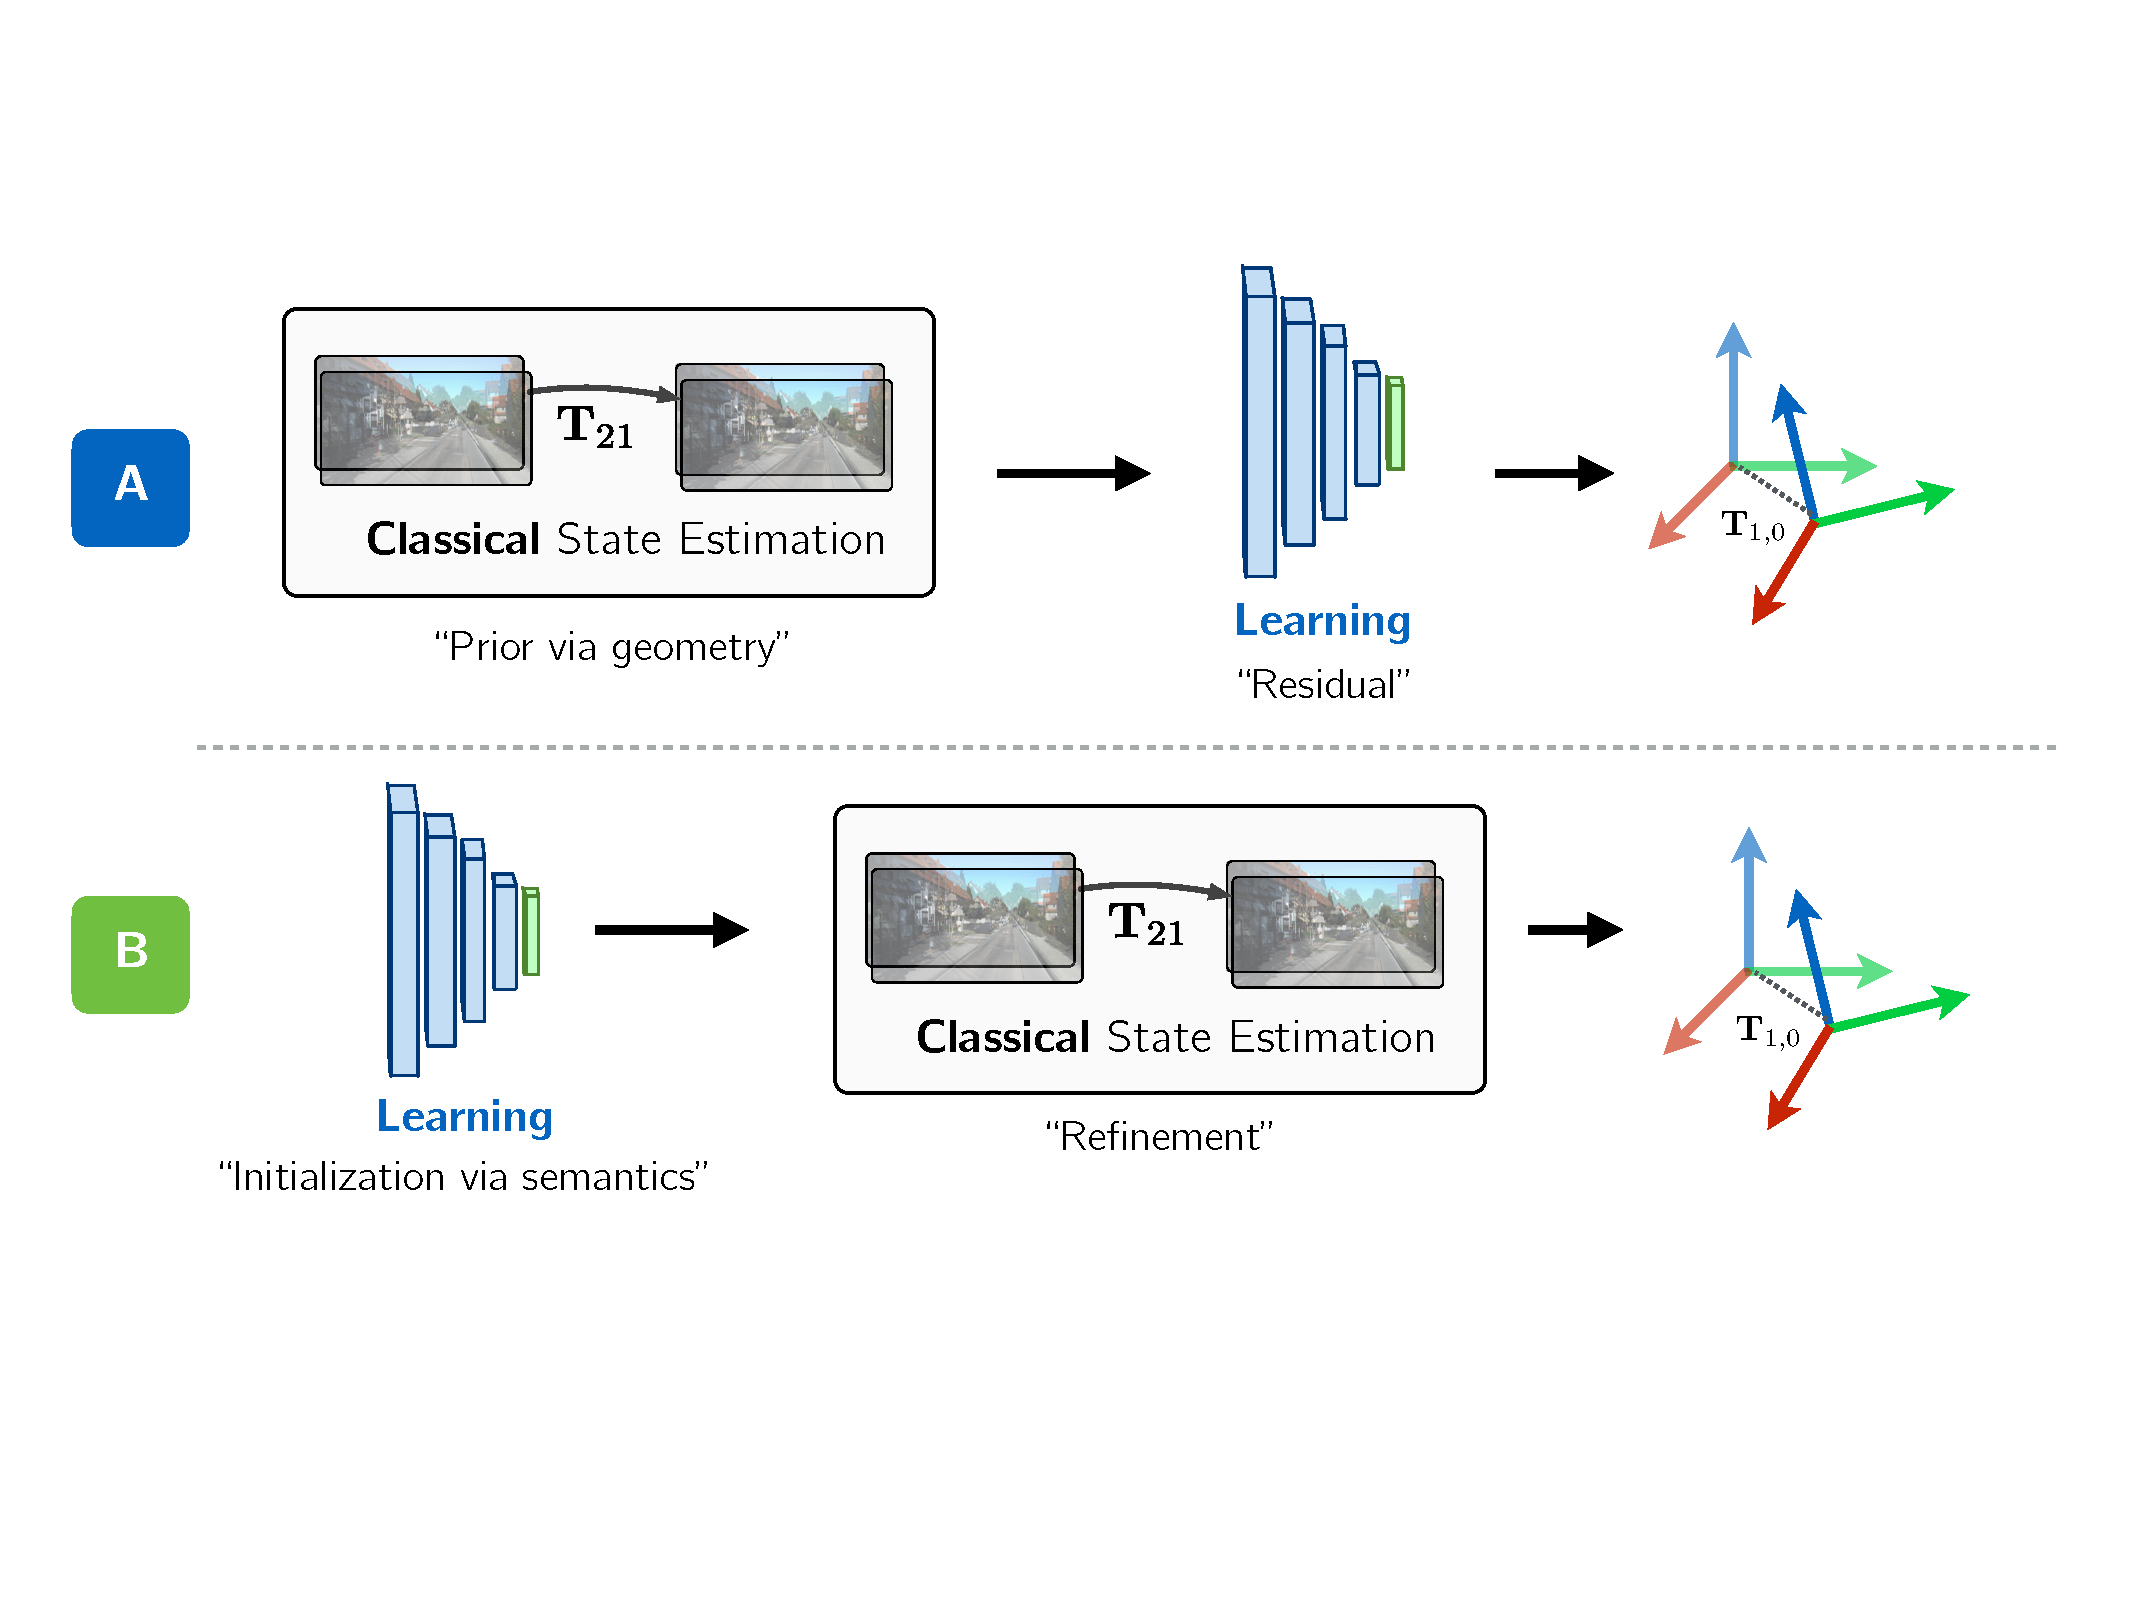
\includegraphics[width=0.98\textwidth]{conclusion/learning_as_prior.pdf}
		\caption{Two different ways to incorporate learning with classical pipelines. The first is by using pipelines as a \textit{prior} which can then be corrected by learned approaches, while the second is use learning as an initialization which can then be \textit{refined} by classical techniques.}
  	\label{fig:conc_learning_as_prior}
\end{center}
\end{figure}


There are many avenues for future work. For instance, although the fusion of pipelines with pseudo-sensors can significantly improve localization performance in a given environment, there are few guarantees that the final estimates are accurate and consistent.

A potential thread of future work addresses this deficiency by developing more tightly-coupled perception systems that can be ‘certified’ to produce globally-optimal solutions while still being robust to adverse environmental effects. To do this, we propose that another way to fuse learned models with classical optimization techniques. Instead of treating the learning as a way to incorporate residuals (as much of this thesis is), we propose that we use learning as initializations, or priors, that are more invariant to effects like large view-point changes and have the ability to generalize to large-scale environments (\Cref{fig:conc_learning_as_prior}). By incorporating these learned ‘priors’ into an optimization framework, we can leverage recently-developed theory on convex relaxations (e.g., that presented in \cite{Rosen2019-kk}) to ensure that the final localization and mapping results are ‘optimal’, in the sense that they are the global minima of a maximum-likelihood-based loss, and ‘safe’, in the sense that they provide consistent uncertainty estimates even in the presence of unmodelled effects. 

\section{Final Remarks}

The German Philosopher Georg Hegel had a particular dialectic method that involved a triad: a thesis, antithesis and synthesis.
Somewhat curiously, this \textit{thesis} has been an attempt at a \textit{synthesis} of the thesis posed by classical visual egomotion, and the antithesis posed by data-drive end-to-end learning techniques.
My hope is that the synthesis based on the concept of \textit{pseudo-sensors} will prove to be a fruitful one within the field of state-estimation, and for the broader robotics community at large.